\documentclass[../main.tex]{subfiles}
\begin{document}

\chapter{Quantum Computing: Machine Learning}
\label{sec:fifth}

\section{Basics of quantum computing}\label{sec:basic_qc}
Quantum computing uses the occurrences of quantum mechanics to process and manipulate information. Quantum computing has endless of possibilities to speed up computations when solving certain problems.
But to understand the beauty of machine learning within quantum computing, one needs to know the basics of quantum computing first, here comes a short summary with the most important key elements to grasp the article. For a deeper dive into the theory on quantum computing, it would be worth starting here \cite{10.5555/1972505}.

The key element when comparing classical computers with quantum computers is the comparison between classical bits and qubits. A classical computer uses bits to handle and manipulate information, where each bit can be either 0 or 1. A quantum computer on the other hand uses qubits. Qubits have the possibility of taking the form of superpositions between the original bits of 0 and 1, often explained by using the Blocks sphere in \autoref{fig:blochsphere}. A qubit can be a superposition of two states, \ensuremath{\alpha|0\rangle+\beta|1\rangle} where \ensuremath{|\alpha|^2+|\beta|^2=1} which opens up the possibility of having multiple states at once.

\begin{figure}[h]
    \centering
    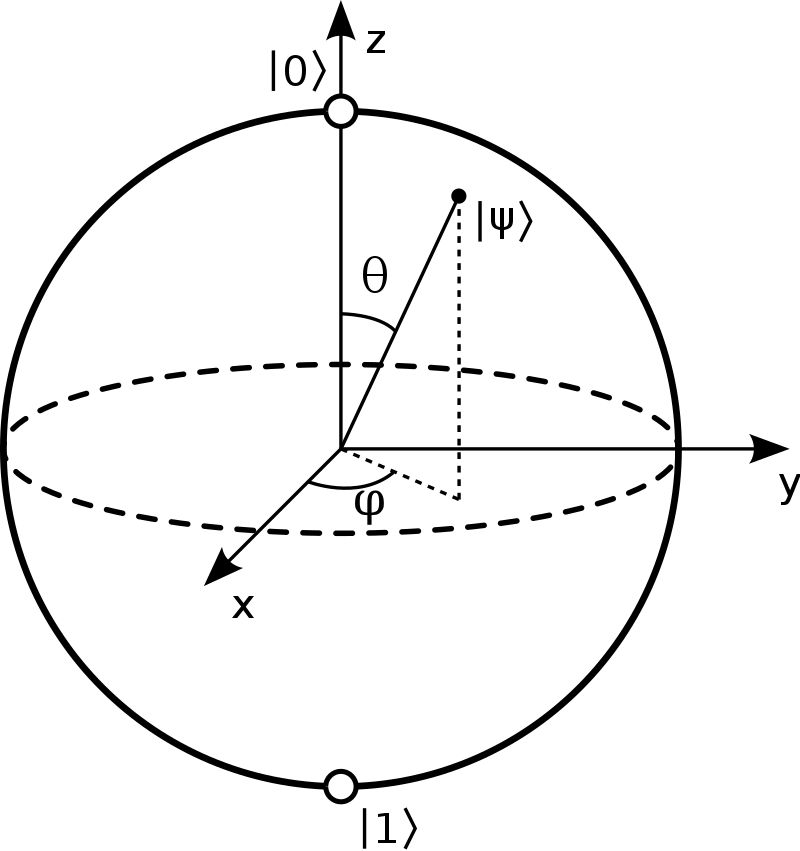
\includegraphics[width=0.5\textwidth]{figures/blochsphere.png}
    \caption{The Bloch sphere showing a geometrical representation of the quantum states of a qubit. A qubit can take a position anywhere on the Bloch sphere of the following form: \ensuremath{|\psi\rangle=cos\frac{\theta}{2}|0\rangle+e^{i\phi}sin\frac{\theta}{2}|1\rangle}, while classical bits are prohibited from taking positions other than the top and bottom. Figure from \cite{blochsphere_fig}}
    \label{fig:blochsphere}
\end{figure}


\subsection{Basis}
All operations on qubits can be expressed mathematically. Therefore defining a basis of two possible qubit states as orthogonal vectors are only natural. The two states a qubit can have when being observed are \ensuremath{|0\rangle=[1,0]^T} and \ensuremath{|1\rangle=[0,1]^T}. Where \ensuremath{\langle1|0\rangle=0} and \ensuremath{\langle0|0\rangle=1} due to basis states being orthogonal. The basis states expands into \ensuremath{|00\rangle=[1,0,0,0]^T}, \ensuremath{|01\rangle=[0,1,0,0]^T}, \ensuremath{|10\rangle=[0,0,1,0]^T} and \ensuremath{|11\rangle=[0,0,0,1]^T} when having two qubits, which naturally increases the vector size the same pattern when adding more qubits. Linear combinations of the different states are also possible, making superpositions as follows:
\begin{equation}
    |\psi\rangle=\alpha|0\rangle+\beta|1\rangle
\end{equation}
Where \ensuremath{|\alpha|^2+|\beta|^2=1}.

Multiple qubits can be expressed as tensor products of the qubits, the following way:
\begin{equation}
    |\psi_1 \rangle \otimes |\psi_2\rangle... \otimes |\psi_n\rangle=|\psi_1 \psi_2 ... \psi_n\rangle
\end{equation}

\subsection{Quantum circuits}
Quantum circuits consists of quantum wires transferring information. The information is then manipulated by letting some quantum logical gate also called a quantum gate, act on the current state. A quantum circuit could for instance look like the following example:

\begin{equation*}
    \Qcircuit @C=2.5em @R=0.8em {
    \lstick{\ket{0}} &\gate{H}   & \qw              &  \ctrl{1}          & \targ    & \ctrl{2}&\qw  \\
	\lstick{\ket{0}} & \gate{H}  & \gate{Rz(\theta)}&  \targ             & \ctrl{-1}& \ctrl{1}&\qw   \\
	\lstick{\ket{0}} &\gate{H}   & \qw              &  \gate{Ry(\theta)} & \qw      & \targ   & \meter
    }
\end{equation*}

Each horizontal line is called a quantum wire, and each of these represents time evolving from left to right. Each quantum wire represents a qubit which can be altered and manipulated. The start point \ensuremath{\ket{0}} represents the initial state of the qubit, while the end of the qubit represents the quantum state after the quantum gates have acted on the quantum states. When going from left to right, the quantum states encounters some quantum gates represented by boxes containing a letter or just some circles and dots, which unveils the type of gate it is. These quantum gates are the operators which alter the quantum states. Vertical lines between quantum wires shows the presence of controlled gates between the two connected wires. Some quantum gates will be discussed in further details in the next subsection. The last part of the third qubit in the drawn circuit, reveals that the measurement of a qubit will happen here. The results from the measurement then reveals which state the last qubit is in. By measuring the same qubit multiple times gives the probability of having the state in either state \ensuremath{\ket{0}} or \ensuremath{\ket{1}} \cite{cite_circuit_explained}.

\subsubsection{Quantum Logical Gates \cite{Qiskit_book}}
\label{sec:not}

Quantum logical gates or quantum gates which they also are called are different ways of manipulating the information in quantum circuits. Quantum gates are expressed mathematically by matrices. There are infinite many matrices, which makes it possible to manipulate quantum states infinite different ways in theory. Some quantum states are more popular than others, lets have a look at some of the most frequently used ones.

The \textbf{Pauli gates} are often used within quantum circuits. The Pauli X-gate or NOT gate which it is also named can be thought of as a rotation around the x axis \ensuremath{\pi} radians. The NOT gate are represented by the following matrix and bracket:
\begin{equation}
    X=\begin{bmatrix}
    0 & 1\\
    1 & 0
    \end{bmatrix}
    =|0\rangle\langle1|+|1\rangle\langle 0|
\end{equation}
Which interchanges the labels between the two qubit states the following way: 
\begin{equation}
    X|0\rangle=|1\rangle
\end{equation}

The Pauli Y-gate can be thought of as a rotation around the y axis \ensuremath{\pi} radians. The Y-gate are represented by the following matrix and bracket:
\begin{equation}
    Y=\begin{bmatrix}
    0 & -i\\
    i & 0
    \end{bmatrix}
    =-i|0\rangle\langle1|+i|1\rangle\langle 0|
\end{equation}
Which maps \ensuremath{|0\rangle} to \ensuremath{i|1\rangle} and \ensuremath{|1\rangle} to \ensuremath{-i|0\rangle}. the following way:
\begin{align}
        Y|0\rangle=&i|1\rangle\\
        Y|1\rangle=&-i|0\rangle
\end{align}

The Pauli Z-gate works the same way as the other Pauli gates. The Z-gate are represented as a rotation around the z axis \ensuremath{\pi} radians. The Z-gate are represented by the following matrix and bracket:
\begin{equation}
    Z=\begin{bmatrix}
    1 & 0\\
    0 & -1
    \end{bmatrix}
    =|0\rangle\langle0|-|1\rangle\langle 1|
\end{equation}
Which maps \ensuremath{|1\rangle} to \ensuremath{-|1\rangle} and works as an identity operator on \ensuremath{|0\rangle} states the following way:
\begin{align}
        Z|0\rangle=&|0\rangle\\
        Z|1\rangle=&-|1\rangle
\end{align}

But since there exists operators that rotates the quantum states around certain axis by \ensuremath{\pi} radians, there must also exist rotational operators that rotate the qubits an arbitrary amount of radians. In fact the \textbf{rotational operator gates} does this exactly. By inserting a parameter \ensuremath{\theta} one can rotate the quantum states around the x, y, or z axis by that many radians. The rotational operators are given by the following matrices:
\begin{align}
    R_{x}(\theta)=&\exp (-i X \theta / 2)=\left[\begin{array}{cc}
\cos (\theta / 2) & -i \sin (\theta / 2) \\
-i \sin (\theta / 2) & \cos (\theta / 2)
\end{array}\right]\\
R_{y}(\theta)=&\exp (-i Y \theta / 2)=\left[\begin{array}{cc}
\cos (\theta / 2) & -\sin (\theta / 2) \\
\sin (\theta / 2) & \cos (\theta / 2)
\end{array}\right]\\
R_{z}(\theta)=&\exp (-i Z \theta / 2)=\left[\begin{array}{cc}
\exp (-i \theta / 2) & 0 \\
0 & \exp (i \theta / 2)
\end{array}\right]
\end{align}
Where the subscript indicates which axis the rotation is happening along.

The \textbf{Hadamard gate} also called a H-gate are one of the most common quantum gates used. The H-gate are represented by the following matrix and bracket:
\begin{equation}
    H=\frac{1}{\sqrt{2}}\begin{bmatrix}
    1 & 1\\
    1 & -1
    \end{bmatrix}
    =\frac{|0\rangle+|1\rangle}{\sqrt{2}}\langle0|+\frac{|0\rangle-|1\rangle}{\sqrt{2}}\langle1|
\end{equation}
Which maps \ensuremath{|0\rangle} to \ensuremath{\frac{|0\rangle+|1\rangle}{\sqrt{2}}} and \ensuremath{|1\rangle} to \ensuremath{\frac{|0\rangle-|1\rangle}{\sqrt{2}}}. The following way:
\begin{align}
        H|0\rangle=&\frac{|0\rangle+|1\rangle}{\sqrt{2}}\\
        H|1\rangle=&\frac{|0\rangle-|1\rangle}{\sqrt{2}}
\end{align}

\textbf{Controlled quantum gates} are quantum gates that acts on two or more qubits when the criteria of another quantum state are satisfied. The quantum state that needs to satisfy the condition is the controlled gate. An example of a popular controlled gate are the well known CNOT which is a controlled NOT gate. The CNOT on two qubits controls if the first qubit is in state \ensuremath{|1\rangle}. If the controlled qubit possess the state, the NOT gate will act on the second qubit mapping \ensuremath{|0\rangle} to \ensuremath{|1\rangle} and opposite. If the controlled qubit does not contain the criteria state, the CNOT will not act on the state, and instead act as an identity operator. Controlled gates are expressed in quantum circuit diagrams as vertical lines between two or more qubits as in figure \autoref{fig:cnot}, where the dark dots are the control qubits and the other are the gate that potentially acts on the state.

\begin{figure}[h]
    \centering
    \subfloat{\scalebox{2}{%
    \Qcircuit @C=1.4em @R=1.8em {
	    & \ctrl{1} & \qw \\
	    & \gate{X} & \qw
    }}}
    \hspace{15pt}
    \subfloat{\scalebox{2}{%
    \Qcircuit @C=1.4em @R=2.em {
	    & \ctrl{1} & \qw \\
	    & \targ & \qw
    }}}
\hspace{15pt}
    \subfloat{\scalebox{2}{%
    \Qcircuit @C=1.4em @R=1.6em {
	    & \ctrl{1} & \qw \\
	    & \gate{Ry(\theta)} & \qw
    }}}
    \caption{Some controlled quantum gates. a) A controlled NOT gate, called a CNOT. b) Also a CNOT but a slightly different visual appearence but does the same as a controlled NOT gate. c) A controlled Ry gate.}
    \label{fig:cnot}
\end{figure}

\subsubsection{Quantum circuit depth}
The more quantum gates a circuit has, the deeper it is. Quantum circuit depth is the longest path in the cirquit along the quantum wires. Because a quantum state is evolving through time as quantum gates is manipulating the information, time complexity is also used to reefer to the depth or the time steps needed to execute the cirquit. 

The depth of quantum cirquits is based on the fact that keeping quantum states stable for longer periods of time is quiet hard, hence circuits need to be short enough to stay stable during the process. The circuit needs to be complex enough to give satisfactory results, but still be simple enough to keep the circuit depth within sensible restrictions, this is way time complexity of a circuit often is the bottleneck when performing quantum computations.


\subsection{Parameterized Quantum Circuits}
\label{sec:PQC}
Parameterized quantum circuits also called PQCs are quantum circuits consisting of one or more quantum gates that are dependent of some variational parameter. Most often multiple quantum gates that depends of some parameter(s) is put together into a circuit which is used as an ansatz. The ansatzes used in this article will be revealed in section \ref{sec_ansa}.

So how is PQCs connected to supervised learning? Shortly summarised, supervised learning aims to learn trends from data that can be generalized to predict other unseen data. In search of the perfect generalisation of data, the machine learning models need to adjust to training data by optimizing the parameters decreasing the loss which is computed from the prediction estimates and the true labels.

Using this same approach by having the PQC which is dependent on some parameters, predict an output and optimize the parameters used in the circuit gives a machine learning approach to PQCs. To read more about machine learning and PQCs feel free to have a look here \cite{Benedetti_2019}.

\subsubsection{Encoders}
Encoding the information that is going to be manipulated in quantum circuits is the first part of the quantum circuits and therefore crucial. There are multiple ways of encoding the data e.g. basis encoding, amplitude encoding, qsample encoding etc. Different encoding methods can be studied in \cite[ch.~5]{10.5555/3309066}.

A way of encoding the data which will also be done in this thesis, is by having every qubit start off with a Hadamard gate splitting the quantum state into a superposition which is then acted on by a \ensuremath{Rz(x)} gate. The clue on encoding classical data into quantum states lays here, because the input \ensuremath{x} will be the classical feature data. The encoding part of the ansatzes used be as follows:

\begin{equation*}
    \Qcircuit @C=2.5em @R=0.8em {
    \lstick{\ket{0}} &\gate{H}  & \gate{Rz(x_1)} &   \qw  \\
	\lstick{\ket{0}} & \gate{H}  &\gate{Rz(x_2)}   & \qw   \\
	\lstick{\vdots}  &  \vdots        & \vdots    & \\
	\lstick{\ket{0}} &\gate{H}  & \gate{Rz(x_n)}    &  \qw
    }
\end{equation*}

Where n is the number of qubits. By rewriting each feature into a \ensuremath{Rz(x)} quantum gate which is dealt its own qubit, the needed qubits is therefore equal to the number of features, excluding possible qubits used for measuring.

\subsubsection{Ansatzes}
\label{sec_ansa}
Ansatzes used in quantum computations are parts of quantum circuits which is assumed to mimic the behaviour of some function. Making the ansatz more complex opens up the possibility of reaching more parts of the Hilbert space where all quantum states resides. Making really large and complex quantum circuits is difficult due to quantum states being quiet unstable over time, which is why ansatzes must avoid being too complex. In this article, two ansatzes will evaluated. 

An ansatz could for instance consist of rotational operators \ensuremath{Ry(\theta)} along each qubit, which is then followed by some entangling between the qubits using controlled not gates between every pairwise qubit as follows:

\begin{equation*}
    \Qcircuit @C=1.5em @R=0.8em {
    \lstick{\ket{\psi_1}} & \gate{Ry(\theta_1)} & \ctrl{1}&  \qw      & \hdots   &\qw&\gate{Ry(\theta_{n+1})} \\
	\lstick{\ket{\psi_2}} & \gate{Ry(\theta_2)} & \targ   &  \ctrl{1} &  \hdots  & \qw&\gate{Ry(\theta_{n+2})}   \\
	\lstick{\vdots}  &  \vdots             & \qw     &  \targ    &  \hdots  & \ctrl{1}&\vdots\\
	\lstick{\ket{\psi_n}} & \gate{Ry(\theta_n)} & \qw     &  \qw      &   \hdots & \targ &\gate{Ry(\theta_{2n})}
    }
\end{equation*}

Where \ensuremath{\boldsymbol{\theta}} is the variational parameters that needs to be optimized and n is the number of qubits. When more variational parameters are used, the ansatz adds more \ensuremath{Ry(\theta)} gates following the same pattern.


\begin{comment}
The second ansatz will be referred to as "ansatz 2" throughout the article, and consists of the rotational operator \ensuremath{Ry(\theta)} along each qubit as in ansatz 1, but the entanglement in ansatz 2 is a bit more complicated. The \ensuremath{Ry(\theta)} operators are followed by controlled gates controlling all qubits above them as follows:

\begin{equation*}
    \Qcircuit @C=1.5em @R=0.8em {
    \lstick{\ket{\psi_1}} & \gate{Ry(\theta_1)} & \ctrl{1}&  \ctrl{2}  &\qw      &\ctrl{3}&\qw     &\qw      &\hdots  &\qw     &\gate{Ry(\theta_{n+1})}\\
	\lstick{\ket{\psi_2}} & \gate{Ry(\theta_2)} & \targ   &  \qw       &\ctrl{1} &  \qw   &\ctrl{2}&\qw      &\hdots  &\qw     &\gate{Ry(\theta_{n+2})}\\
	\lstick{\ket{\psi_3}} & \gate{Ry(\theta_3)} & \qw     &  \targ     &\targ    &  \qw   &\qw     &\ctrl{1} &\hdots  &\qw     &\gate{Ry(\theta_{n+3})}\\
	\lstick{\vdots}  &  \vdots             & \qw     &  \qw       &\qw      &\targ   & \targ  & \targ   &\hdots  &\ctrl{1}&        \vdots\\
	\lstick{\ket{\psi_n}} & \gate{Ry(\theta_n)} & \qw     &  \qw       &\qw      &\qw     & \qw    &  \qw    &\hdots  &\targ   &\gate{Ry(\theta_{2n})}
    }
\end{equation*}

Where \ensuremath{\boldsymbol{\theta}} is the variational parameters that needs to be optimized and n is the number of qubits. When more variational parameters are used, the ansatz adds more \ensuremath{Ry(\theta)} gates following the same pattern.
\end{comment}

Notice that the input states of the circuit is \ensuremath{\ket{\psi_x}} since the input of the ansatz-part of the circuit is the already altered quantum states from the encoder.

\subsubsection{Entanglement of the qubits}
The last part of a PQCs is the entangling part which entagles all qubits together, making it possible for the qubits to affect eachothers quantum state. The remarkable thing about quantum entanglement is that affecting a qubit might make rise to a change in another qubit, which is one of the main reasons quantum computing is such a powerful tool.

The entangling part is an extra part of the quantum circuit which is appended onto the ansatz. A way of entangling the example ansatz could for instance be a controlled not gate controlling all other qubits except the target qubit which is the last qubit. A measurement could then be performed on the last qubit, giving the probability \ensuremath{|c_1|^2} of having the qubit in state \ensuremath{\ket{1}}, which can be used as a classification prediction between class \ensuremath{\ket{0}} and class \ensuremath{\ket{1}}.

\begin{comment}
For ansatz 2, the entanglement is just a continuation of the controlled not gates from the same ansatz. Which means that the middle part from the ansatz is composed to the end of the quantum circuit. A measurement is then performed on the last qubit, giving the probability \ensuremath{|c_1|^2} of having the qubit in state \ensuremath{\ket{1}}, which the same way as for ansatz 1 can be used as a classification mesurement.
\end{comment}


\section{Quantum Nearest Neighbours}
\label{sec:qnn}
\todo[inline]{This section is from earlier report, rewrite it to match the thesis, especially the discussion part}
Quantum Nearest neighbours is based on the same strategy as in section \ref{sec:knn}, but with some smaller implementation differences to make the method suitable for quantum computing. This section is based on the example provided in \cite[ch.~1]{10.5555/3309066}

To use the nearest neighbours method with quantum computers, the first step is naturally to do a little preprocessing of the data. The data is first and foremost normalised to one. This way the data is only described by the angles according to the origin since all samples have the same unit length from the origin.

The next step is to encode the data. A safe and secure way to encode the data is to use amplitude encoding. The amplitude vector is made by concatenating the features of the data, and the normalised data. After the amplitude vector is made, the number of qubits needed to perform the algorithm are decided.

The next step is to apply the quantum operations. When performing the nearest neighbours method the Hadamard is the quantum operator to use. The Hadamard operator acts on the amplitude vector, which creates a new amplitude vector. Since the Hadamard operator maps the states into superpositions, the new amplitude vector contains a lot of different states and values which will be rejected or accepted when the measurement starts.

Then the rejection sampling starts by measuring the first qubit, rejecting and setting the value to zero if the state are \ensuremath{|1\rangle}, hence only keeping the accepted states \ensuremath{|0\rangle} or opposite, which then are normalised.

The ancilla qubit is measured, and the amplitudes in similar states are squared and added together, which results in the final probabilities to find the unknown datapoint within the given category. A theoretical example of the method will be explored in section \ref{KNNimp}.

\subsection{Quantum computing case}
Then it is time to have a look at the same example if implemented on a quantum computer. Classifying the unknown sample in the small dataset from table \ref{tab:dataset_tit} by using nearest neigbours with quantum computing is done by following the recipe in section \ref{sec:qnn}. The first step is to preprocess the data by having the vector of ticket price and room number normalized. This way all the samples will have the same length from the center, making the angles the only relevant descripting of the sample placements. The dataset normalized to unit length can be seen in table \ref{tab:dataset_tit2}.

\begin{table}[ht]
\caption{Table showing some samples used for creating a small dataset. The dataset is showing the ticket price the travelers paid and the room number before normalisation(BN), and the same information after normalising the data to unit length(AN) assuming the maximum ticket price and room number was 10000 and 2500 respectively. The survival column shows the survival of the travelers, 1 means survival while 0 means no survival.}
\centerline{
\begin{tabular}{ cccccc } 
\toprule
Traveler & Price (BN)& Room number (BN) & Price (AN) & Room number (AN) & Survival \\
\midrule
1        &   8500 & 0910 & 0.921 & 0.390 & 1\\
2        &   1200 & 2105 & 0.141 & 0.990 & 0\\
3        &   7800 & 1121 & 0.866 & 0.500 & \\
\bottomrule
\end{tabular}}
\label{tab:dataset_tit2}
\end{table}

The new values can be plotted the same way as in the classical case, giving the plot in figure \ref{fig:knn_qua}

\begin{figure}[ht]
    \centering
    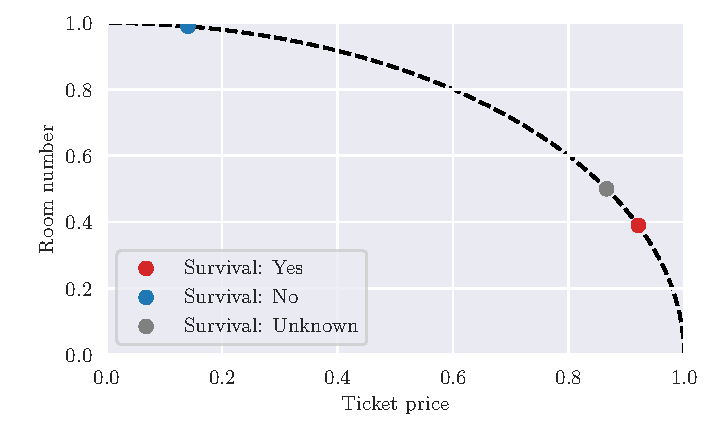
\includegraphics{figures/Cqnn.pdf}
    \caption{Plot of the ticket price and room number for the three travelers, after normalizing the data to unit length.}
    \label{fig:knn_qua}
\end{figure}

Next step follows and the data is encoded into amplitude vectors. The features of the data are appended to the same vector, and the unknown sample are appended twice, which makes the unknown sample data added and subtracted to both the known samples, which gives the following vector:
\begin{equation}
\alpha=\frac{1}{2}(0.921, 0.39, 0.141, 0.99, 0.866, 0.5, 0.866, 0.5)^T
\end{equation}

Where the factor \ensuremath{\frac{1}{2}} at the start is a normalisation factor, to ensure that the sum of the squared amplitudes equals 1. 

Since three qubits have the possibilliy of having \ensuremath{2^3=8} states, one more qubit is added representing the two categories, which results in the following amplitude vector having \ensuremath{2^4=16} states. The states added from the fourth qubit are currently only zeros, leaving the following amplitude vector:
\begin{equation}
\alpha=\frac{1}{2}(0, 0.921, 0, 0.39, 0.141, 0, 0.99, 0, 0, 0.866, 0, 0.5, 0.866, 0, 0.5, 0)^T
\end{equation}
Which can be written in the form of quantum states as follows:
\begin{equation}
\begin{split}
|\psi_{0}\rangle=\frac{1}{2}(&0.921|0001\rangle+0.390|0011\rangle+0.141|0100\rangle+0.990|0110\rangle\\+&0.866|1001\rangle
+0.500|1011\rangle+0.866|1100\rangle+0.500|1110\rangle)
\end{split}
\end{equation}

Now that the preprocessing and encoding is done the Hadamard transformation can begin. The Hadamard operator acts on the current state, which adds and subtracts the last four amplitudes to the first four amplitudes which gives the following results:
\begin{equation}
\begin{split}
|\psi_{1}\rangle=H|\psi_{0}\rangle=\frac{1}{2}((&0.921+0.866)|0001\rangle+(0.390+0.500)|0011\rangle\\+(&0.141+0.866)|0100\rangle+(0.990+0.500)|0110\rangle\\+(&0.921-0.866)|1001\rangle
+(0.390-0.500)|1011\rangle\\+(&0.141-0.866)|1100\rangle+(0.990-0.500)|1110\rangle)
\end{split}
\label{eq:sub2}
\end{equation}

Which written in a more compact way equals:
\begin{equation}
\begin{split}
|\psi_{1}\rangle=H|\psi_{0}\rangle=&0.8935|0001\rangle+0.445|0011\rangle
+0.5035|0100\rangle+0.745|0110\rangle\\
+&0.0275|1001\rangle-0.055|1011\rangle
-0.3625|1100\rangle+0.245|1110\rangle
\end{split}
\label{eq:sub}
\end{equation}

Now the next step is to reject half of the states due to the fact that half of the samples has the unknown sample data summed to their amplitude, while the rest has the same data subtracted, which is more clear having a look at equation \eqref{eq:sub2}. There is only need for one linear combination containing the unknown sample data, which is why half of the data is rejected. It is easy to see from equation \eqref{eq:sub} that the states that needs to be rejected are the states which has the first qubit in state \ensuremath{|1\rangle}, else the amplitude is set to 0. Then the resulting states named \ensuremath{\psi_2} are as follows:
\begin{equation}
|\psi_{2}\rangle=\frac{1}{\chi}(0.8935|0001\rangle+0.4450|0011\rangle
+0.5035|0100\rangle+0.7450|0110\rangle)
\end{equation}
Which equals the following after normalisation.
\begin{equation}
|\psi_{2}\rangle=0.665|0001\rangle+0.331|0011\rangle
+0.375|0100\rangle+0.555|0110\rangle)
\end{equation}

As mentioned at the start of the subsection, the fourth qubit was added to be used as a label indicator. Which means that states with equal fourth qubits represents the same category. Then the amplitudes of the states in the same category can be used to compute the probability of finding the unknown sample in each of the category by adding the squared amplitudes within each class as follows:
\begin{equation}
p(|xxx0\rangle)=|0.375|^2+|0.555|^2\approx0.448
\end{equation}

Which means that the probability of finding the unknown sample as a traveler that did not survive equals 0.448. While the probability of finding the traveler as a survivor equals:
\begin{equation}
p(|xxx1\rangle)=1-p(|xxx0\rangle)=|0.665|^2+|0.331|^2\approx0.552
\end{equation}

Which means that the unknown passenger is classified as a survivor, which is the same as for the classical case of nearest neighbours.

\subsubsection{QNN vs. classical NN}
The results of the calculations done in section \ref{KNNimp}, showed that computing a nearest neighbour method for both a classical and quantum computing case managed to classify the unknown samples correct. In addition the probability of classifying the unknown case within each category were also the same when using equation \eqref{eq:knnweight} and \eqref{eq:knnprob} according to \cite[ch.~1]{10.5555/3309066}. Which makes sense due to the Hadamard operator being an universal classical gate, the proof can be seen here \cite{cite:hadamardproof}.

Comparing the complexity of both the methods reveals that the quantum implementation of nearest neighbours is more efficient the more samples the dataset contains because the quantum states possible are proportional to \ensuremath{2^n} using n qubits. The quantum implementation of the nearest neighbours used one Hadamard transformation and two measurements, which is quite few operations remembering the fact that with just these few manipulations it is possible to classify unknown samples. 

The bad thing in the classical case is that the length to its neighbours need to be computed for each sample, which can be quiet computationally expensive when dealing with a large number of samples, and even more expensive if \ensuremath{k} is high and a lot of the neighbours are contributing to the classification of each unknown sample.

In the quantum computing case, there might be some loss of information when normalizing the data to unit length. The loss of information could be that samples within the same classes might get pushed away from each other when forcing each sample along the same unit circle. Observing the example with quantum nearest neighbours showed that in this case loss of information was not a problem.


\section{Variational quantum Boltzmann machine}
Maybe use this as the section headline, then ite under.
Add a subsection proposing a neural network finding the coefficients.

\section{Variational quantum imaginary time evolution}
\label{sec:VarITE}
In a variational quantum Boltzmann machine(VarQBM) Gibbs states need to be prepared beforehand, a way to do this is to use a method called variatioanal quantum imaginary time evolution(VarQITE), the details on VarQBM and how to prepare the Gibbs states using varQITE will be revealed later in the theory section, but firstly the details on classical imaginary time evolution(ITE) and varQITE need to be laid out first.

ITE is quiet usual when looking for ground state energies and studying quantum systems using classical computers \cite{McArdle_2019}. Following the explanation in \cite{VQB:litteraturelist} ITE is based on starting of with an initial quantum state $\ket{\psi_0}$. ITE is then used to evolve $\ket{\psi_0}$ into quantum state $\ket{\psi_\tau}$ at time $\tau$ using the following time-independent Hamiltonian $H$:

\begin{equation}
H=\sum_{i=0}^{p-1} \theta_{i} h_{i}
\end{equation}

Where $\theta_i$ is some real coefficients and $h_i$ represent some Pauli matrix. The evolved quantum state can then be denoted as the following:

\begin{equation}
\left|\psi_{\tau}\right\rangle=C(\tau) e^{-H \tau}\left|\psi_{0}\right\rangle
\end{equation}

Where $C(\tau)$ is the normalization factor given as the following:

\begin{equation}
C(\tau)=1 / \sqrt{\operatorname{Tr}\left[e^{-2 H \tau}\left|\psi_{0}\right\rangle\left\langle\psi_{0}\right|\right]}
\end{equation}

The evolution of the quantum state is represented by the Wick-rotated Schrödinger equation. Wick rotations is used to solve mathematical problems by substituting real variables with imaginary variables, done here by introducing imaginary time \cite{PhysRev.96.1124}. The Wick-rotated Schrödinger equation is represented by the following differential equation:

\begin{equation}
\frac{d\left|\psi_{\tau}\right\rangle}{d \tau}=-\left(H-E_{\tau}\right)\left|\psi_{\tau}\right\rangle
\label{eq:wick_SE}
\end{equation}

With $E_{\tau}=\left\langle\psi_{\tau}|H| \psi_{\tau}\right\rangle$. According to Zoufal, Lucchi and Woerner \cite{VQB:litteraturelist}, the terms in the Hamiltonian representing the largest eigenvalue decays faster than the terms representing the small eigenvalues. Due to this, as long as there is some overlap between the eigenvalue and the ground state, the eigenvalue found is in fact the ground state of the system when $\tau \rightarrow \infty$ \cite{VQB:litteraturelist}. Further on one can prepare the Gibbs states by having a finite limit $\tau=1 / 2\left(\mathrm{k}_{\mathrm{B}} \mathrm{T}\right)$ on the time evolution.

\todo[inline]{Why is that? The 'accordning to..' part}

Now that the main details of ITE is unveiled, it is time to jump into varQITE. The idea of varQITE is to minimize the energy using McLachlan's variational principle \cite{doi:10.1080/00268976400100041} by introducing a parameterized trial state $\ket{\psi_\omega}$ in addition to representing the time evolution by some parameters $\omega(\tau)$.

Since varQITE is intended to be run on quantum computers, a quantum circuit is defined as $V(\tau)=U_q(\omega_q)\hdots U_1(\omega_1)$. An initial quantum state is also defined as $\ket{\psi_{in}}$ which is the input state. The trial state is the written as follows:

\begin{equation}
\left|\psi_{\omega}\right\rangle:=V(\omega)\left|\psi_{\text {in }}\right\rangle
\end{equation}

Rewriting \autoref{eq:wick_SE} by throwing all terms to the left hand side and factorising the evolved state the equation can be written as follows
\begin{equation}
    \left(\frac{d}{d \tau}+H-E_{\tau}\right)\left|\psi_{\tau}\right\rangle=0
\end{equation}

Then by switching the evolved state $\ket{\psi_\tau}$ with the trial state $\ket{\psi_\omega}$ and multiplying with a factor $\delta$ to account for the error that arises when $\ket{\psi_\tau} \neq \ket{\psi_\omega}$, one arrives at McLachlan's variational principle:

\begin{equation}
\delta \|\left(\frac{d}{d \tau}+H-E_{\tau}\right)\left|\psi_{\omega}\right\rangle \|=0
\label{eq:mcvar}
\end{equation}

Now McLachlan's variational principle is a central part in determining the parameters $\omega(\tau)$. Then solving \autoref{eq:mcvar} leads to the following system of linear equations:

\begin{equation}
A \dot{\omega}=C
\label{eq:AwC}
\end{equation}

Where $\dot{\omega}=\frac{d\omega}{d \tau}$ and A and C is given as the following:

\begin{equation}
\begin{aligned}
&A_{p q}(\tau)=\operatorname{Re}\left(\operatorname{Tr}\left[\frac{\partial V^{\dagger}(\omega(\tau))}{\partial \omega(\tau)_{p}} \frac{\partial V(\omega(\tau))}{\partial \omega(\tau)_{q}} \rho_{\mathrm{in}}\right]\right) \\
&C_{p}(\tau)=-\sum_{i} \theta_{i} \operatorname{Re}\left(\operatorname{Tr}\left[\frac{\partial V^{\dagger}(\omega(\tau))}{\partial \omega(\tau)_{p}} h_{i} V(\omega(\tau)) \rho_{\mathrm{in}}\right]\right)
\end{aligned}
\label{eq:A_and_C}
\end{equation}

With $Re(\cdot)$ being the real part of the expression and $\rho_{\mathrm{in}}=\left|\psi_{\mathrm{in}}\right\rangle\left\langle\psi_{\mathrm{in}}\right|$. To evaluate $A$ and $C$ in varQITE, some expectation values need to be computed by using some quantum circuit composed following some rules, more on the evaluation and form of the quantum circuit will be unveiled in the next section.

Demanding that the matrices $U(\omega)$ within  $V(\omega)$ are arbitrary unitary matrices $U(\omega)$ it is possible to evaluate the expressions $A$ and $C$. The reason for this is that all unitary matrices can be written as $U(\omega)=e^{i M(\omega)}$ where $M(\omega)$ is a parameterized Hermitian matrix. The Hermitian matrices can then be rewritten as weighted sums of pauli terms as explained in \cite{VQB:litteraturelist}:

\begin{equation}
M(\omega)=\sum_{p} m_{p}(\omega) h_{p}
\end{equation}
Where $m_{p}(\omega) \in \mathbb{R}$ and $h_p$ is given as $h_{p}=\bigotimes_{j=0}^{n-1} \sigma_{j, p}$, $j$ being which qubit the operation is performed on and $\sigma_{j, p} \in\{I, X, Y, Z\}$. The gradient of $U_k(\omega_k)$ is then defined as follows:

\begin{equation}
\frac{\partial U_{k}\left(\omega_{k}\right)}{\partial \omega_{k}}=\sum_{p} i \frac{\partial m_{k, p}\left(\omega_{k}\right)}{\partial \omega_{k}} U_{k}\left(\omega_{k}\right) h_{k_{p}}
\end{equation}.

No that the steps of varQITE is defined, the last step remaining is letting the parameters evolve with time, which can be done multiple ways, for instance with an explicit Euler the following way:

\begin{equation}
\omega(\tau)=\omega(0)+\sum_{j=1}^{\tau / \delta \tau} \dot{\omega}(\tau) \delta \tau
\end{equation}

\subsection{Evaluation of expression- $A$ and $C$ and their gradients}
The expressions $A$ and $C$ from \autoref{eq:A_and_C} used in varQITE is a couple of expressions which is composed on the following form:

\begin{equation}
\operatorname{Re}\left(e^{i \alpha} \operatorname{Tr}\left[U^{\dagger} V \rho_{\mathrm{in}}\right]\right)
\label{eq:trial_state_basic_form}
\end{equation}

By computing the expectation value of an observable $Z$ it is possible to evaluate the two expressions in \autoref{eq:A_and_C} by sampling from $Z$ with respect to the circuit in \eqref{circ_fig:appendix} according to \cite{VQB:litteraturelist} and \cite{McArdle_2019}\cite{Yuan_2019}\cite{Somma_2002}.

\begin{equation}
    \centering
    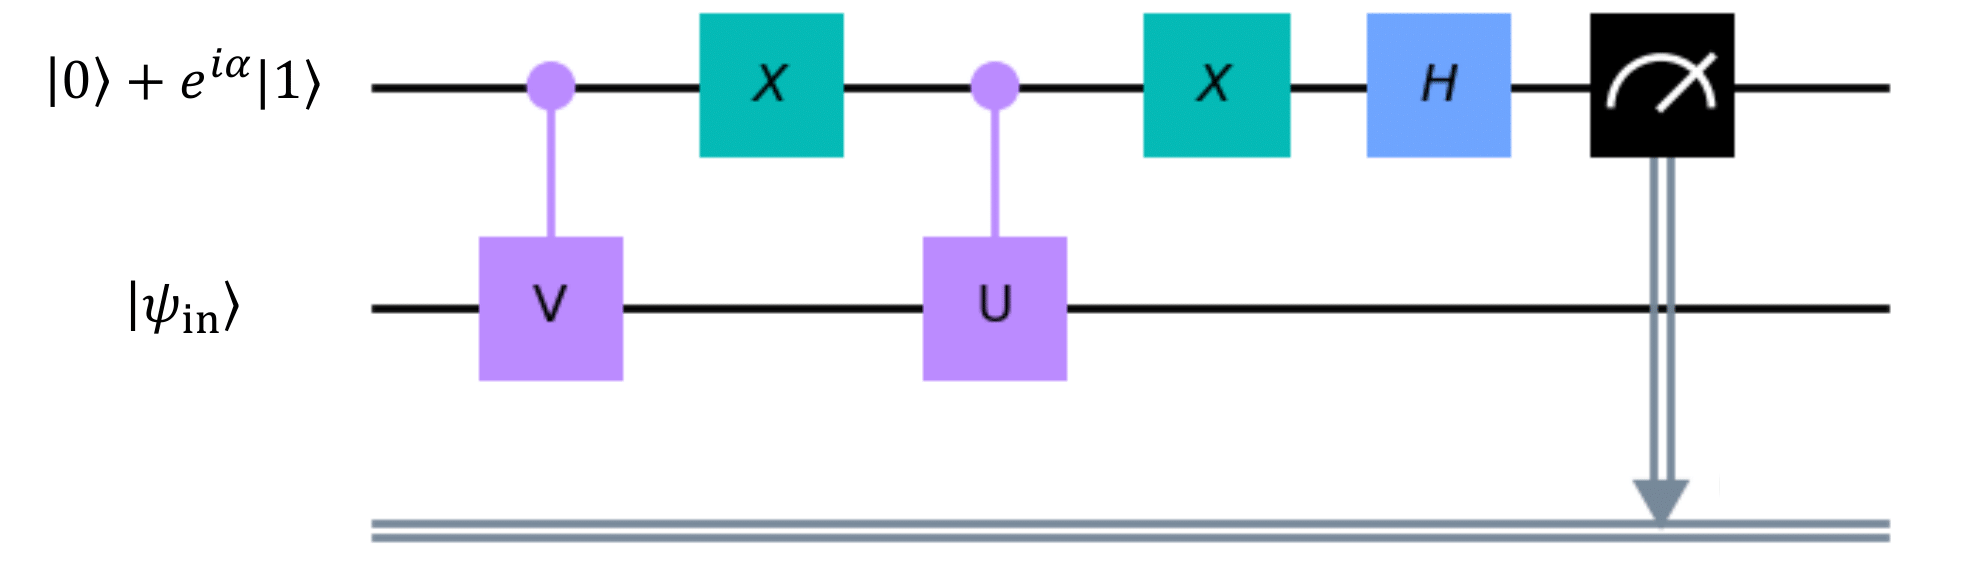
\includegraphics[width=1\textwidth]{figures/eval_circ_fig-1.png}
    \label{circ_fig:appendix}
\end{equation}

\todo[inline]{Might draw the same figure with qcircuit. Should a circuit be an equation or a figure?}

To make the phase factor $e^{i\alpha}$ go along with the expressions in \autoref{eq:A_and_C}, the first qubit is initialized a bit differently for the two expressions. Expression $A$ is initialised with an H gate, while $C$ is initialised with an H- followed by an S gate. 

It is also important to remember that since the trial states are constructed via Pauli rotations the matrix $U(\omega)$ can be written as follows:

\begin{equation}
U(\omega)=R_{\sigma_{l}}(\omega)
\end{equation}

Where $\sigma_{l} \in\{X, Y, Z\}$. Which gives the following derivative:

\begin{equation}
\frac{\partial U(\omega)}{\partial \omega}=-\frac{i}{2} \sigma_{l} R_{\sigma_{l}}(\omega)
\end{equation}

Further on the terms of the derivatives of expression $A$ and $C$ can be written on the same form as \autoref{eq:trial_state_basic_form}. The derivative of expression $A$ can be expressed as follows:

\begin{equation}
\begin{aligned}
\partial_{\theta_{i}} A_{p, q}(\tau)&= \sum_{s} \frac{\partial \omega_{s}(\tau)}{\partial_{\theta_{i}}} \operatorname{Re}\left(\operatorname { T r } \left[\left(\frac{\partial^{2} V^{\dagger}(\omega(\tau))}{\partial \omega_{p}(\tau) \partial \omega_{s}(\tau)} \frac{\partial V(\omega(\tau))}{\partial \omega(\tau)_{q}}\right.\right.\right. \\
&\left.\left.\left.+\frac{\partial V^{\dagger}(\omega(\tau))}{\partial \omega(\tau)_{p}} \frac{\partial^{2} V(\omega(\tau))}{\partial \omega_{q}(\tau) \partial \omega_{s}(\tau)}\right) \rho_{\mathrm{in}}\right]\right)
\end{aligned}
\end{equation}

And the derivative of expression $C$ can be expressed as follows:

\begin{equation}
\begin{aligned}
\partial_{\theta_{j}} C_{p}(\tau)=& -\operatorname{Re}\left(\operatorname{Tr}\left[\frac{\partial V^{\dagger}(\omega(\tau))}{\partial \omega(\tau)_{p}} h_{j} V(\omega(\tau)) \rho_{\mathrm{in}}\right]\right) \\
&-\sum_{i, s} \theta_{i} \frac{\partial \omega_{s}(\tau)}{\partial_{\theta_{j}}} \operatorname{Re}\left(\operatorname { T r } \left[\left(\frac{\partial V^{\dagger}(\omega(\tau))}{\partial \omega_{p}(\tau)} h_{i} \frac{\partial V(\omega(\tau))}{\partial \omega_{s}(\tau)}\right.\right.\right. \\
&\left.\left.\left.+\frac{\partial^{2} V^{\dagger}(\omega(\tau))}{\partial \omega_{p}(\tau) \partial \omega_{s}(\tau)} h_{i} V(\omega(\tau))\right) \rho_{\mathrm{in}}\right]\right)
\end{aligned}
\end{equation}

Where $\alpha$ is set equal to $\frac{\pi}{2}$ and $0$ in the expressions corresponding to $A$ and $C$ respectively. 


\section{Quantum Boltzmann machine}
Before jumping into VarQBM, regular QBM which lays the basis of VarQBM needs to be explained. 
\begin{comment}
QBM can be seen as a kind of a plain transformation of a classical Boltzmann machine into an approach which can be implemented on a quantum computer.
\end{comment}

As mentioned in \autoref{sec:BM} a BM consists of hidden and visible units. A QBM on the other hand consists of visible and hidden qubits. A QBM can be defined as a parameterized Hamiltonian $H_{\theta}=\sum_{i=0}^{p-1} \theta_{i} h_{i}$ where $\theta\in\R^p$ and $h_{i}=\bigotimes_{j=0}^{n-1} \sigma_{j, i}$ with $\sigma_{j, i} \in\{I, X, Y, Z\}$ acting on qubit $j$.

The visible qubits determines the output of the QBM, which makes it natural to define the probability of measuring a configuration $v$ with respect to the projective measurement $\Lambda_{v}=|v\rangle\langle v| \otimes I$ on the Gibbs state given by:

\begin{equation}
\rho^{\text {Gibbs }}=\frac{e^{-H_{\theta} /\left(\mathrm{k}_{\mathrm{B}} \mathrm{T}\right)}}{Z}
\end{equation}

Where $Z=\operatorname{Tr}\left[e^{-H_{\theta} /\left(\mathrm{k}_{\mathrm{B}} \mathrm{T}\right)}\right]$ which gives the probability of measuring $\ket{v}$ as follows:

\begin{equation}
p_{v}^{\mathrm{QBM}}=\operatorname{Tr}\left[\Lambda_{v} \rho^{\mathrm{Gibbs}}\right]
\end{equation}

As mentioned before, the purpose of a QBM is to compute probability distributions such that sampling $\rho^{\text {Gibbs }}$ corresponds to sampling from the classical target distribution with as much overlap between the probabillity distributions possible. The loss used in QBM is the same as in classical Boltzmann machines:

\begin{equation}
L=-\sum p_{v}^{\mathrm{data}} \log p_{v}^{\mathrm{QBM}}
\label{eq:Loss_QBM}
\end{equation}

With $p_{v}^{\text {data }}$ being the probability of having $v$ taking place in the training data. The loss function naturally depends on the variational parameters $\theta$, such that the gradients are computed with respect to the same parameters. The difference between a regular QBM and a VarQBM which will be implemented in this thesis is that in VarQBM the gradient of the loss function is computed analytically.

That was a bit on regular QBMs, feel free to have a look at the following article for a more in depth explanation on QBMs \cite{Amin_2018}. 

Even though there are multiple similarities between QBMs and VarQBMs, there is still some key differences. Now that general QBMs are covered it is time to move further into the details of VarQBM. The steps of a VarQBM is visualized in figure \ref{fig:varQBMsteps}.

\begin{figure}[h]
    \centering
    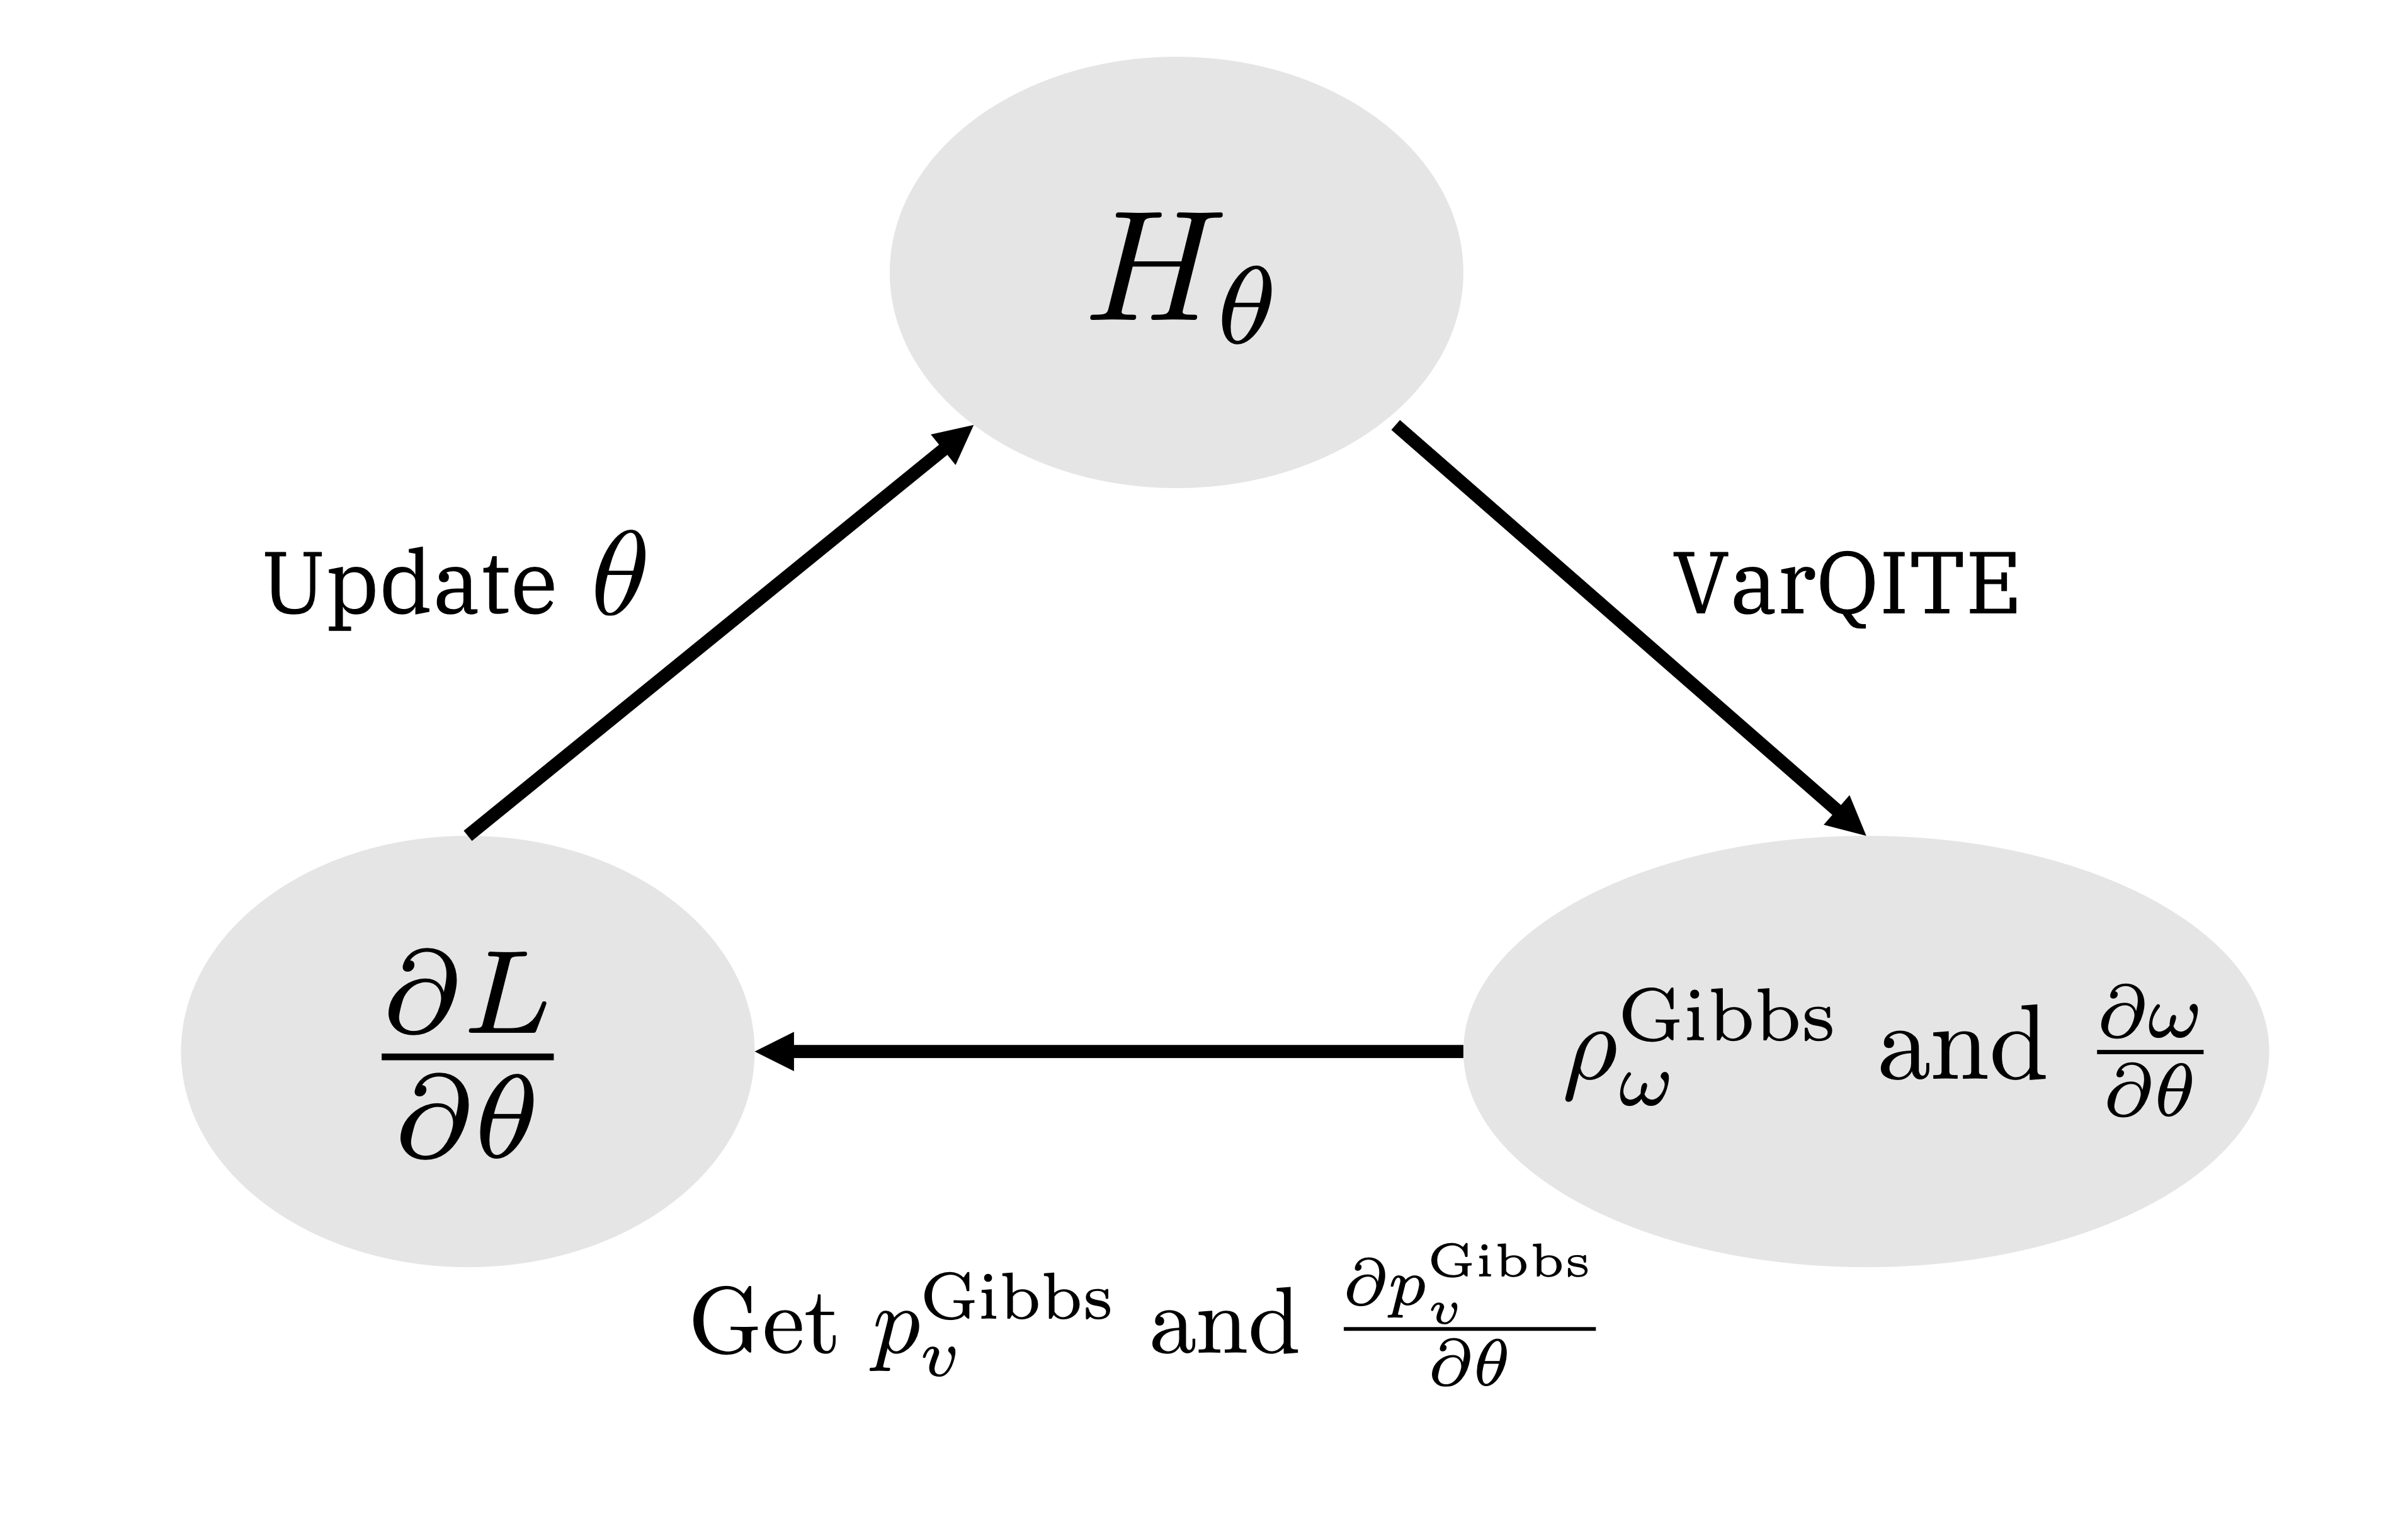
\includegraphics[width=0.65\textwidth]{figures/varqbm.png}
    \caption{Steps of VarQBM, first step is to approximate the Gibbs states using VarQITE. Next step is to find the gradient of the loss function which is then used to update the variational parameters according to some classical optimization algorithm. Figure from \cite{VQB:litteraturelist}}
    \label{fig:varQBMsteps}
\end{figure}

\subsection{Preparation of Gibbs states with VarQITE}
Lets have a look at how it is possible to prepare the Gibbs state $\rho^{\text {Gibbs }}$ using Variational Quantum Imaginary Time Evolution. The Gibbs state expresses a probability density operator. The density operator defines the configuration space of a system in thermal equilibrium \cite{GibbsElementaryPI} \cite{VQB:litteraturelist}. So how is $\rho^{\text {Gibbs }}$ prepared? There are multiple different ways proposed which consists of strategies like Quantum Phase Estimation \cite{Temme_2011, Yung_2012, Poulin_2009}, evaluation of quantum thermal averages \cite{Motta_2019, brandao2019finite, kastoryano2016quantum} and more. As said earlier VarQITE will be used for this task, due to the fact that this scheme is compatible with near-term quantum computers in addition to having a clear knowing of the needed ancilla qubits.

So lets walk through the steps of preparing the Gibbs state $\rho^{\text {Gibbs }}$, also here a lot of the walk through will follow \cite{VQB:litteraturelist}. First step is to set up the quantum circuit $V(\omega)$, $\omega \in \mathbb{R}^{q}$ and initialize the variational parameters to satisfy the following initial state:

\begin{equation}
\left|\psi_{0}\right\rangle=V(\omega(0))|0\rangle^{\otimes 2 n}=\left|\phi^{+}\right\rangle^{\otimes n}
\end{equation}

With $\ket{\phi^+}$ being the Bell state:

\begin{equation}
\left|\phi^{+}\right\rangle=\frac{1}{\sqrt{2}}(|00\rangle+|11\rangle)
\end{equation}

By introducing two n-qubit sub-systems $a$ and $b$ where the first qubit of the Bell states starts of in $a$ and the second qubit in $b$, an effective Hamiltonian $H_{eff}$ is defined as follows:

\begin{equation}
H_{eff}=H_{\theta}^{a}+I^{b}
\end{equation}

With the superscript denoting which sub-system the operator acts upon. Since sub-system $b$ will be a maximally mixed state \cite{VQB:litteraturelist}, it will act as an ancillary qubit system, where tracing the sub-system gives the following:

\begin{equation}
\operatorname{Tr}_{b}\left[\left|\phi^{+}\right\rangle^{\otimes n}\right]=\frac{1}{2^{n}} I
\end{equation}

Next step is to find the approximation which is the goal of VarQITE. This is done by starting the propagation until time $\tau=1/2(k_b T)$ is reached with respect to the effective Hamiltonian. Doing this gives the following state:

\begin{equation}
\left|\psi_{\omega}\right\rangle=V(\omega(\tau))|0\rangle^{\otimes 2 n}
\end{equation}

Which is used to compute $\rho_\omega^{\text {Gibbs }}$ as follows:

\begin{equation}
\rho_{\omega}^{\mathrm{Gibbs}}=\operatorname{Tr}_{b}[|\psi(\omega(\tau))\rangle\langle\psi(\omega(\tau))|] \approx \frac{e^{-H_{\theta} /\left(\mathrm{k}_{\mathrm{B}} \mathrm{T}\right)}}{Z}
\end{equation}

And we arrive at the Gibbs state approximation using VarQITE.

\subsection{Variational Quantum Boltzmann Machine}
Finally it is time to unveil the VarQBM algorithm, and at the same time give an overview and connect the different parts together. As mentioned earlier, the goal of the method is to be able to reproduce probability distributions by optimizing some variational parameters $\theta$ such that when sampling from the generated distribution using Gibbs states prepared with VarQITE approximates the training data.

The variational parameters are optimized by minimizing \autoref{eq:Loss_QBM} the following way:

\begin{equation}
\min _{\theta} L=\min _{\theta}\left(-\sum_{v} p_{v}^{\mathrm{data}} \log p_{v}^{\mathrm{QBM}}\right)
\end{equation}

Where the gradient is computed with respect to each variational parameter the following way:

\begin{equation}
\frac{\partial L}{\partial \theta_{i}} =\frac{\partial\left(-\sum_{v} p_{v}^{\text {data }} \log p_{v}^{\mathrm{QBM}}\right)}{\partial \theta_{i}}=-\sum_{v} p_{v}^{\mathrm{data}} \frac{\partial p_{v}^{\mathrm{QBM}} / \partial \theta_{i}}{p_{v}^{\mathrm{QBM}}}
\end{equation}

Which is computed by using the chain rule, which gives the following expression for the gradient:

\begin{equation}
\frac{\partial p_{v}^{\mathrm{QBM}}}{\partial \theta_{i}} =\frac{\partial p_{v}^{\mathrm{QBM}}}{\partial \omega(\tau)} \frac{\partial \omega(\tau)}{\partial \theta_{i}}=\sum_{k=0}^{q-1} \frac{\partial p_{v}^{\mathrm{QBM}}}{\partial \omega_{k}(\tau)} \frac{\partial \omega_{k}(\tau)}{\partial \theta_{i}}
\end{equation}

With 

\begin{equation}
\frac{\partial p_{v}^{\mathrm{QBM}}}{\partial \omega_{k}(\tau)}=\frac{\partial \operatorname{Tr}\left[\Lambda_{v} \rho_{\omega}^{\mathrm{Gibbs}}\right]}{\partial \omega_{k}(\tau)}
\end{equation}

Which can be found by utilizing gradient methods like the parameter-shift rule \cite{crooks2019gradients}. By differentiating \autoref{eq:AwC}, $\frac{\partial \omega_{k}(\tau)}{ \partial \theta_{i}}$ can be found. The derivative of \autoref{eq:AwC} is given as follows:

\begin{equation}
A\left(\frac{\partial \dot{\omega}(\tau)}{\partial \theta_{i}}\right)=\frac{\partial C}{\partial \theta_{i}}-\left(\frac{\partial A}{\partial \theta_{i}}\right) \dot{\omega}(\tau)
\end{equation}

Which can solved with respect to the wanted expression $\frac{\partial \dot{\omega}(\tau)}{ \partial \theta_{i}}$, by evaluating the expression for every time step used in VarQITE. Further on by utilizing a differentiation method like explicit Euler method for instance, the following expression is given:

\begin{equation}
\begin{aligned}
\frac{\partial \omega_{k}(\tau)}{\partial_{\theta_{i}}} &=\frac{\partial \omega_{k}(\tau-\delta \tau)}{\partial_{\theta_{i}}}+\frac{\partial \dot{\omega}_{k}(\tau-\delta \tau)}{\partial_{\theta_{i}}} \delta \tau \\
&=\frac{\partial \omega_{k}(0)}{\partial_{\theta_{i}}}+\sum_{j=1}^{\tau / \delta \tau} \frac{\partial \dot{\omega}_{k}(j \delta \tau)}{\partial_{\theta_{i}}} \delta \tau
\end{aligned}
\end{equation}

The optimizer is then utilized to optimize the variational paramters. In this thesis the Adam optimize will be chosen to optimize the VarQBM.

\section{Expectation values of Hamiltonian quantum circuits}
When optimizing a trial circuit representing some ansatz to minimize some expectation energy, the ansatz naturally needs to be applied to the Hamiltonian to compute the expectation value of the energy, but how is this done when measuring qubits only provides a sampling probability between 0 and 1?

In context of Boltzmann machines all Hamiltonians compatible with Boltzmann distributions can be used and written as a sum of Pauli products\cite{VQB:litteraturelist}. Computing the expectation energy of a Hamiltonian given on the following form is actually fairly straightforward:

\begin{equation*}
H=\sum_{i=0}^{p-1} \theta_{i} h_{i},
\end{equation*}

with $p$ being the number of Hamiltonian terms in the Hamiltonian, $\theta$ being some factor and $h_i$ being a quantum gate. Now having an Hamiltonian act on a quantum state $\ket{\psi}$ represented as a quantum circuit used to find the expectation energy the following way:

\begin{equation}
    \langle E \rangle=\bra{\psi} H \ket{\psi}=\sum_{i=0}^{p-1}\theta_i \bra{\psi}h_i\ket{\psi}.
\label{eq:expect_energy}
\end{equation}

Which shows how the different terms of a Hamiltonian is assessed. But one thing is missing, namely the expectation value of the Hamiltonian terms. First and foremost $h_i$ is a tensor product of pauli gates. Pauli matrices are $2 \times 2$ matrices which looks as follows:

\begin{equation}
&\sigma_{\mathrm{x}}=\left(\begin{array}{cc}
0 & 1 \\
1 & 0
\end{array}\right), \quad
&\sigma_{\mathrm{y}}=\left(\begin{array}{cc}
0 & -i \\
i & 0
\end{array}\right), \quad
&\sigma_{\mathrm{z}}=\left(\begin{array}{cc}
1 & 0 \\
0 & -1
\end{array}\right).
\end{equation}

When measuring quantum circuits, the measured quantum states are forced out of superposition and into some eigenstate, therefore a quantum circuit are measured multiple times and averaged over the possible states measured to get a statistical distribution of the possibilities to measure the different states, often referred to as sampling probabilities. The number of times measured is often referred to as shots. The most common basis to measure quantum circuits in is the $Pauli-Z basis$ with eigenstates $\ket{0}$ and $\ket{1}$, there is no problem using other bases as well. The eigenvalues of eigenstate $\ket{0}$ and $\ket{1}$ equal $1$ and $-1$ respectively. When summing the terms of \autoref{eq:expect_energy} the sampling probability of a given state is then multiplied by its corresponding eigenvalue $-1$ or $1$, before multiplied by the factor $\theta$.

Further on the Hamiltonian terms often consists of tensor products of multiple Pauli gates, which means that there are multiple qubits hence even more possible quantum states to collapse into. When evaluating a Hamiltonian term  $Z_0 Z_1$ meaning the first and second qubit consists of a Z gate each, there is four possible quantum states when measuring each of the qubits, since each qubit can take values of $0$ or $1$. The eigenvalues of each qubit is multiplied by eachother resulting in the addition or subtraction of the sampling probability of the given state. The same approach follows when utilizing Hamiltonians consisting of terms existing of an arbitrary number of qubits.

Even though the Pauli-Z basis is most often used to measure quantum circuits, the Hamiltonian terms might not always consist of Pauli-Z matrices. So how is quantum gates other than Pauli-Z gates measured in the Z basis? This is simply solved by rotating the statevector of the quantum state to point in the direction of the computational basis and measure same way as for Pauli-Z gates.

The easiest way to explain this process is probably by showing an example of circuits used. Lets assume some Hamiltonian is given by the following:

\begin{equation}
    H=Z+X+Y,
\end{equation}

which gives the following expectation value:

\begin{align*}
    \bra{\psi}H\ket{\psi}&=\bra{\psi}Z\ket{\psi}+\bra{\psi}X\ket{\psi}+\bra{\psi}Y\ket{\psi}\\
    &=\bra{\psi}Z\ket{\psi}+\bra{\psi}H^\prime ZH^\prime \ket{\psi}+\bra{\psi}H^\prime SZH^\prime S^\dagger\ket{\psi}\\
    &=\bra{\psi}Z\ket{\psi}+\bra{\psi H^\prime}Z\ket{H^\prime \psi}+\bra{\psi H^\prime S}Z\ket{H^\prime S^{\dagger}\psi},
\end{align*}

where $H^\prime$ is the Hadamard gate. Which shows that by adding a few gates to the quantum circuit it is possible to measure the contributions of $X$ and $Y$ oriented quantum states. The circuits used to measure the different contributions of Z,X and Y looks as follows:
\begin{equation*}
    \Qcircuit @C=1.5em @R=0.8em {
    \ket{\psi} & & \qw & \qw &\qw & \qw &\meter}
\end{equation*}
\begin{equation*}
    \Qcircuit @C=1.5em @R=0.8em {
    \ket{\psi} & & \qw & \qw&\gate{H} & \meter}
\end{equation*}
\begin{equation*}
    \Qcircuit @C=1.5em @R=0.8em {
    \ket{\psi} & & \gate{S^\dagger}&\gate{H} & \meter}
\end{equation*}

Where the qubits are used to find $\bra{\psi}Z\ket{\psi}$, $\bra{\psi}X\ket{\psi}$ and $\bra{\psi}Y\ket{\psi}$ respectively.

\section{Jordan-Wigner transformation}
Write some general theory on JW

Write about how the qubits are sorted based on orbital, spin and spacial orbital

\subsection{Jordan-Wigner transformation of the pairing Hamiltonian}

Rewrite the second quantized pairing Hamiltonian into qubits form using JW

\section{Theory on variational quantum simulations? Got some nice litterature on the topic at the start of the thesis}



\end{document}